%-----------------------------------------------------------------------------------------
\clearpage
\section{Literature Review}
%-----------------------------------------------------------------------------------------
\subsection{Brief Introduction to Machine Learning and Neural Networks}
To first understand Distributed Machine Learning you must first understand the
fundamentals of machine learning and neural networks. 

There are many machine learning methods some requiring training data which we
call supervised and some being able to find patterns in data without being given
solutions called unsupervised. \cite{alpaydin2020introduction} An example of a
supervised system may be predicting house prices, using multiple factors about
each house (market data, geographic area, square footage etc.) to come to a
conclusion about what the house could sell for. This would be trained using data
of previously sold houses to predict current ones. An example of an unsupervised
system could be identification of new plant species. This could be done by
taking as many features of a plant as possible, then apply a clustering
algorithm to see if there are two distinct clusters in the data. If there were
then that would suggest two different plant species. Neural networks tend to
focus on supervised learning and use a form gradient descent called Stochastic
Gradient Descent.

Many machine learning algorithms use a cost function to measure how well or
badly they are solving a problem, these algorithms use parameters which are
internal variables of a machine learning model and define how they solve the
problem. If you map \(costFunction(x)\), where \(x\) is the model parameter, for
every \(x\) value. Then a graph will be produced \(y = costFunction(x)\), the
lowest point on the graph will be the global minimum. There may be other troughs
higher than the global minimum these are called local minimums. A global minimum
represents the lowest value of the cost function which indicates the parameter
values produce the best solution for your problem. Initial model parameters are
often randomised, meaning they may start at a high point on the cost function
graph, the goal is to get to the lowest point possible. To do this you must
\textit{descend} down the \textit{gradient} to a local minima, the algorithm
that does this is called gradient descent for that very reason. This often
happens in little steps after the observation of each piece of data. However it
is computationally expensive to step down the gradient after each example. It is
more efficient to calculate the average step of a randomised selection of data.
This is know as Stochastic Gradient Descent.

Neural networks are structures that can perform multi-variable gradient descent
when provided with training data. Neural networks are comprised of layers of
interconnected neurons in a lattice like structure. Each neuron holds parameter
information the adjusting of which through stochastic gradient descent leads to
the solving of a problem through reaching the local minimum of the cost
function.

\subsection{The Communication Issue}
Distributed neural networks must communicate with each other in some way in
order to work together. This needs to be formalised to be able to measure the
efficiency of our machine learning system. Parts of this reasoning already
appears in these papers too. \cite{konevcny2016federated ,Ma2017DistributedOptimisation}

If we consider how a neural network operates if we were to run it on a single
node, we could characterise its computation as such:
\begin{equation}
    TIME = I_A (\epsilon) \times T_A 
\end{equation}

Where \(I_A(\epsilon)\) is the number of iterations of the algorithm \(A\) it
takes to reach accuracy \(\epsilon\) and \(T_A\) is the time of each iteration
of the algorithm. Here maximising the convergence per iteration or decreasing
the time an iteration takes will decrease the runtime of the algorithm. In a
distributed setting this equation changes to this:
\begin{equation}
    TIME = I_A (\epsilon) \times (c + T_A)  
\end{equation}
In this equation we have the added variable \(c\), this represents time taken
for communication per iteration. In a distributed setting this will always
remain above a non trivial amount of data. Unfortunately The majority of machine
learning algorithms use a stochastic method which means a very large number of
iterations \((I_A(\epsilon))\) that take a short amount of time (small \(T_A\)).
You can see that no matter how small \(c\) is there will be a significant impact
of the time taken. In fact with a naive approach of communication each iteration
almost certainly \(c > T_A\).

However this view doesn't take into account the possibility that communication
could happen at the same time as an iteration. For example imagine a pipeline of
nodes where each nodes performs an iteration but can communicate its previous
iteration to the next node at the same time. Then the time taken could be
described like so:
\begin{equation}
    TIME = I_A (\epsilon) \times max(c, T_A)
\end{equation}
Here you can see that if you can find a way of making the communication time
equal to the time per iteration. Then \(c\) would have a negligible effect on
the equation.

\subsection{Limited History of Distributed Machine Learning}
One of the first pieces of research into distributed machine learning was
’Distributed Inference for Latent Dirichlet Allocation’ in 2008
\cite{newman2008distributed} One of the first instances of distributed machine
learning  was  used  to  categorise  New York  Times  articles  using  Latent
Dirichlet Allocation (LDA), which identifies the affiliations words have to
certain topics.  While the paper focused on parallelising the algorithm and
running them over multiple artificially isolated cores the results showed that
distributed machine learning could have scalability and didn’t impact the rate
of convergence of the model significantly. This was followed by a paper by Jia
et al. \cite{ParallelTopicModels} which produced much faster results than its
predecessors by using memcache layer in every machine, every machine would
message every other machine with updates of its local parameters to create an
approximate global state, it was mentioned in passing that arranging the nodes
in a star topology and caching the values that passed through it could make the
system more scalable. After this followed a cambrian explosion of work in this
area \cite{Ahmed2012YahooLDA, li2014communication, Dean2012Distbelief,
googlemapreduce2008} culminating in 2014 when the parameter server as it is
known today \cite{LI2014ParameterServers} was produced. This parameter server is
highly sophisticated and flexible accommodating the difference in hardware
components while spending more on computation and less time waiting.



\subsection{Model and Data Parallelism}
\begin{figure}[h]
    \centering
    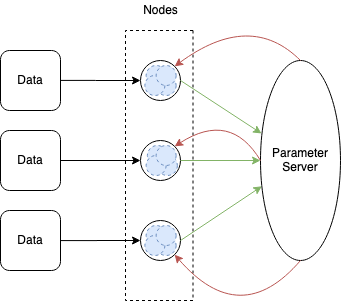
\includegraphics[width=0.4\textwidth]{DataParallel}
    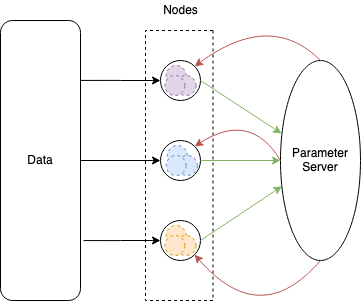
\includegraphics[width=0.4\textwidth]{ModelParallel}
    \caption{Left: Data Parallelism. Right: Model Parallelism. In both diagrams
        the green lines indicate local parameters being sent to the parameter
        server and red lines indicate parameters being sent to the worker nodes.}
\end{figure}
When creating distributed machine learning models there two different methods
for distributing training, model parallelism and data parallelism. These two
methods are not mutually exclusive and can be used in conjunction with one
another, such as in DistBelief. \cite{Dean2012Distbelief}. model parallelism is
when model parameters are split between the nodes. As data parallelism is when
the data is split between the nodes. \cite{Xing2015Petuum} Often with model
parallelism the whole set of training data is passed through each node. While in
data parallelism its common for each node to hold the whole machine learning
model.

The key advantage of model parallelism is that machine learning models can be
far larger as they no longer have to sit on one machine. However this one great
advantage comes with some disadvantages. Some parameters may take more time to
converge than others, this means that at times some nodes may be idle while
others are still converging, so the spread of computation is not equal or
efficient. \cite{Dean2012Distbelief} Because some parameters converge at
different rates a scheduler can be used, which does improve model convergence.
However this requires more computational overhead and communication and reduces
iteration throughput.
\cite{kim2016STRADS}

data parallelism has the benefit that data throughput can be very large, making
processing using this method very fast. However with more nodes the
communication overhead increases as the nodes must communicate the changes in
their model parameters to each other. \cite{elgabli2020gadmm} The nodes can
communicate with each other synchronously, but this means the computation is
only as fast as the slowest node. If the nodes communicate with each other
asynchronously then some of the calculations will be made on out of date model
parameters so training examples may be needlessly wasted.

\subsection{Low Power Hardware, IoT and Mobile Computation}

Historically machine learning algorithms have been focused on high model
accuracy through large models and vast amounts of training data, energy
consumption and efficiency has rarely been taken into consideration. However
with the rise of Internet of Things (IoT) devices and the established ubiquity
of smart phones more data than ever is being produced. Soon this data generation
with exceed the capacity of the internet, and experts estimate that over 90\% of
data will be stored and processed locally. \cite{Chaing2016FogIoT} By extension
this means machine learning algorithms will have to be performed locally too.
This introduces some challenging issues. Modern machine learning algorithms
require vast computational power and large amounts of data. Local devices don't
have the capacity to hold large data sets or the power to compute large machine
learning models in a viable amount of time, while many of them are also battery
powered so power consumption becomes another issue.

% modern solutions for edge computing 
A solution to this is to massively distribute the model over multiple
decentralised nodes. The level of distribution is even greater than that of
centralised compute clusters. In this solution each device computes a model
using its own local data, infrequently (due to network constraints) the model is
shared with a coordination server, which will then distribute the changes across
all nodes in the network. \cite{wang2018EdgeLearning} While this method is
inefficient as the infrequent communications mean that many nodes may do much of
the same work, and the merging of local models into a global one infrequently
may cause loss of information. It still produces a model which converges in a
relatively few rounds of communication. \cite{konevcny2016federated}

% low power solutions
Efforts have been made in techniques to reduce the power memory and storage
needed for machine learning algorithms to operate. One of these is Data Stream
Mining. The idea is that a device can stream the analytics data directly into
the model rather than storing the data in storage for later use.
\cite{garciaMartin2019MLEnergy} This means after the data has been read by the
model it is lost. But that also means that no data needs to be stored, meaning
resources are not spent reading and writing to storage. This has an application
in mobile devices, as they produce data at a low rate through user interaction.
Therefore the model can be build in real time as actions occur. The data
produced on the mobile itself may not be enough to effectively train the model,
but via communication with other users distributed over the network the model
can converge. \cite{konevcny2016federated}

% there has not been much work done in low power distributed setting
From the research available there seems to be research into distributed
computing on local devices, investigation in to power measurements of machine
learning algorithms \cite{wang2018EdgeLearning, konevcny2016federated} and
power reduction of machine learning algorithms on local devices.
\cite{garciaMartin2019MLEnergy} But there is a distinct lack of research into
efficiency of \textit{distributed algorithms} from the perspective of efficiency
and power consumption on local devices. Having a more power efficient
distributed machine learning algorithm, even if the optimisation was marginal on
each device, would have an enormous effect on the output of the system, as many
devices are connected.

